\documentclass[../main.tex]{subfiles}

\begin{document}

Due to the propagation delay of transactions in the network, not all nodes share the same vision of the Tangle at the same time.
This might lead to situations where the validation process lets multiple transactions in conflict with each other join the Tangle.
It is a fundamental assumption of the IOTA white paper that the Tangle itself can indeed contain conflicting transactions.
In case of a conflict, however, the nodes need to decide which transaction(s) should eventually be considered valid, i.e., they need to come to a \emph{consensus} on those conflicting transactions.

In the IOTA white paper this is solely achieved by consistently applying the tip selection algorithm (TSA), i.e., the mechanism used by (honest) nodes to select the transactions to approve, which currently uses a biased random walk. In case of a conflict, this bias will eventually leave all but one of the conflicting branches behind. However, as already stated throughout this document, this approach is only sufficient under the honest transaction majority assumption. Furthermore, the conflict resolution is slow, which leads to leave transactions that chose the ``wrong'' branch behind, creating the need for reattachments.

In this work, we present a novel consensus mechanism which integrates a voting system, helping to deal with the aforementioned issues. Whilst the voting models have their limitations, they have been successfully applied in a wide range of engineering and economical applications~\cite{banisch2010, niu2015, przyby2011}, leading to the emerging science of sociophysics~\cite{castellano2009}. For the sake of presentation, we decouple the consensus in two main components (see also Fig.~\ref{fig:consensus-diagram}):
\begin{itemize}
    \item \textit{Tip selection algorithm.} In Section~\ref{sec:tsa}, we present a few important enhancements to the random walk-based algorithm proposed in the IOTA white paper with the objective of increasing the overall throughput and the robustness against parasite chain and splitting attacks.
    \item \textit{Voting mechanism.} In Section~\ref{sec:voting}, we describe two voting mechanisms where nodes communicate to each other to decide, in case of a conflict, which transaction(s) should be accepted in the Tangle.
\end{itemize}

\begin{figure}[h]
     \centering
     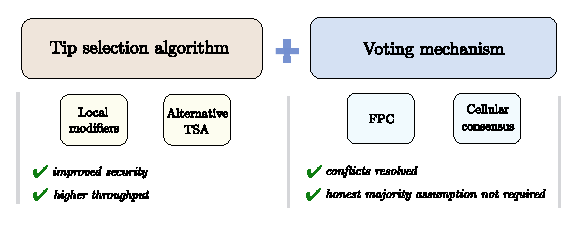
\includegraphics[scale=1.2]{images/consensus-diagram.eps}
     \caption{Our novel consensus mechanism adds a voting layer to improve security and to deal with the honest majority assumption.}
     \label{fig:consensus-diagram}
\end{figure}

\end{document}
